%% ==============================================================================
%%
%%  Document settings and macro definitions
%%
%% ==============================================================================

\documentclass[a4paper,10pt,bibtotoc]{scrartcl}
\usepackage{a4wide,usg}
\usepackage{draftcopy}
\usepackage{upgreek}

\newcommand\sumline[2]{%
  \hbox to \linewidth{%
    \strut
    \parbox[t]{.85\linewidth}{\strut #1\strut}\hss
    \parbox[t]{.15\linewidth}{\raggedleft\strut #2\strut}%
  }
}

\newcommand\kw[0]{$KW$}

%% Do NOT remove: required to extract SVN information
\svnInfo $Id$

%% Adjust page footer
\fancyfoot[LE,LO]{LOFAR-DWG-ICD-XXX: MY-DATATYPE-DATA}
\fancyfoot[RE,RO]{\textsc{lofar} Project}

%% ==============================================================================
%%
%%  Document
%%
%% ==============================================================================

\begin{document}

\title{LOFAR Data Format ICD \\ MY-DATATYPE-DATA \\
  {\normalsize Document ID: LOFAR-DWG-ICD-XXX} \\
  {\normalsize Version 1.00.00} \\
  {\normalsize SVN Repository Revision: \svnInfoMaxRevision} \\
   {\normalsize Persistent DOI: XXXXXX} \\
\author{ \parbox{\linewidth}{\centering S.~ter~Veen, H.~Holties } }
\date{\small{SVN Date: \svnInfoMaxToday}} \\

  
}

\maketitle


\section{Table of contents}
\tableofcontents

\listoffigures

\listoftables

\clearpage

%% ______________________________________________________________________________
%%                                                                  Change record




\input version_numbering




\clearpage

%%_______________________________________________________________________________
%%                                                                   Introduction

\section{Introduction}
\label{sec:introduction}

\subsection{Purpose and scope}
\label{sec:purpose and scope}

This interface control document (ICD) describes the internal structure
of and the interface to the LOFAR time series data as generated by the Transient Buffer Boards (TBB) 
 Time series data -- i.e. the digitised voltage output, as received by the individual
LOFAR dipoles -- represent the primary input data to the CR (Cosmic
Ray) analysis pipeline(s) and have to be considered as the most basic
form in which the received radio signals are present within the LOFAR
system. With the LOFAR 2.0 upgrade, this functionality is known as Transient Buffer (TBuf) as they do not have their own separate board.

This document therefore serves as reference for the
implementation of tools that read and write the data, see \ref{sec:tools}.


\subsection{Applicable Documents}
\input applicable_to_all_documents

\begin{center}
  %% Table head
  \tablefirsthead{
    \hline
    \textsc{Reference} & \textsc{Title} & \textsc{Description} \\
    \hline
  }
  \tablehead{
    \multicolumn{3}{r}{\small \textbf{Applicable documents}
      \textsl{continued from previous page}} \\
    \hline
    \textsc{Reference} & \textsc{Title} & \textsc{Description} \\
    \hline
  }
  %% Table tail
  \tabletail{
    \hline
    \multicolumn{3}{r}{\small\sl continued on next page} \\
  }
  \tablelasttail{\hline}
  %% Table contents
  \bottomcaption[List of documents that apply specifically to this LOFAR Control Document (ICDs)]{List of documents that apply specifically to this LOFAR Control Document (ICDs)
  \label{tab:applicable list}}
  \begin{supertabular}{lp{5.8cm}p{7cm}}
    \shrinkheight{-4.5em}
    \texttt{ICD-001} \cite{lofar.icd.001} & Previous description for LOFAR1 data format. \\
    \hline
  \end{supertabular}
\end{center}

\subsection{Reference applications}
This document serves as reference for the
implementation of tools that read and write the data. A non-extensive list is provided here.

\begin{center}
  %% Table head
  \tablefirsthead{
    \hline
    \textsc{Name} & \textsc{Title} & \textsc{Purpose} \\
    \hline
  }
  \tablehead{
    \multicolumn{3}{r}{\small \textbf{Applicable documents}
      \textsl{continued from previous page}} \\
    \hline
    \textsc{Reference} & \textsc{Title} & \textsc{Description} \\
    \hline
  }
  %% Table tail
  \tabletail{
    \hline
    \multicolumn{3}{r}{\small\sl continued on next page} \\
  }
  \tablelasttail{\hline}
  %% Table contents
  \bottomcaption[List of tools that read and/or write this data format]{
    List of tools that read and/or write this data format.
  \label{tab:applicable list}}
  \begin{supertabular}{lp{4.8cm}p{6cm}}
    \shrinkheight{-4.5em}
    \texttt{DAL} \cite{tools.1} & Data access library & C++ Library to read and write this dataformat. \\
    \texttt{Cosmic Ray Pipeline} \cite{tools.2} & Cosmic Ray Pipeline & Pipeline to analyse cosmic ray data \\
    \texttt{Lightning mapper} \cite{tools.3} & Lightning imager &  3-D imager for lightning \\
    \hline
  \end{supertabular}
\end{center}
%% ______________________________________________________________________________
%%                                                              Section: Overview

\subsection{Overview}
\label{sec:overview}

This document is structured as follows: %
Section \ref{sec:structure} will describe fundamental overall
structure, including a statement of the primary data product format,
HDF5. These conventions will also include names, meaning, and physical
units that may be used to generate and interpret the data files. %
Section \ref{sec:detailed structure} will present a detailed
specification for the data, including a description of the structure
of a LOFAR TBB data naming conventions, units, physical quantities. %

\begin{comment}
This is not a finished document. It needs further definition and clarification in the text of what certain values mean.
\end{comment}

%%_______________________________________________________________________________
%%                                                       Organisation of the data

\clearpage

\section{Organisation of the data}
\label{sec:structure}



\subsection{Conventions}
The following conventions apply to this LOFAR interface control document.

\input types

\input notation


\subsection{Data Structure}

A LOFAR TBB Times-series data file will adhere to the following guidelines:\\

A LOFAR TBB Times-series data file will be defined within the context
of the HDF5 file format.  A LOFAR TBB Time-series HDF5 file structure
will comprise a primary group, a "root group" in HDF5 nomenclature,
which may be considered equivalent to a primary header/data unit (HDU)
of a standard multi-extension FITS file.  This primary group will
consist only of header keywords (“attributes” in HDF5 nomenclature)
describing general properties of an observation, along with pointers
to contained subgroups.  Those subgroups will comprise an arbitrary
number of ``StationGroups'' (see sec~\ref{sec:station group}), where a
Station Group will contain data and meta-data produced by an
individual LOFAR station. Under each Station Group there are one or two more levels
depending on the data taking mode used.

Figure~\ref{fig:TBB_highlevel} shows the basic organisation of the dataset within
the HDF5 format. The hierarchical structure essentially follows the
hierarchical structure of LOFAR itself, i.e. in a top-down approach
from array through stations down to individual dipoles. The grouping
of multiple antennas/dipoles into a station is mirrored by the
collection of dipole datasets into a station group.

\subsubsection{Overview of TBB Groups}

The structure of the file is subdivided into the following four HDF5 group levels, depending on which mode is being used:

\begin{enumerate}
\item \textbf{File Root Group} (\verb|ROOT|). The root level of the file contains the
  majority of associated meta-data, describing the circumstances of
  the observation. These data attributes include observation time
  (start and end), frequency window (high band vs. low band, filters)
  and other important characteristics of the dataset. See
  section \ref{sec:root group} for further details.
\item \textbf{Station Group} (\verb|STATION_{AAKKK}|). This group serves as a
  common container for the separate sub-tables, which take up data from the
  station calibration and the trigger algorithm. 
  The part between \verb|{...}| represents the station name and consists of 2
  characters (upper case) and three digits (e.g. 'CS001' or 'RS106'). 
  See section \ref{sec:station group} for further details.
\end{enumerate}

%%_______________________________________________________________________________
%%                                                    Detailed Data Specification


\subsubsection{Hierarchical structure}
\label{sec:hierarchical structure}

\begin{figure}[htb]
  \centering
  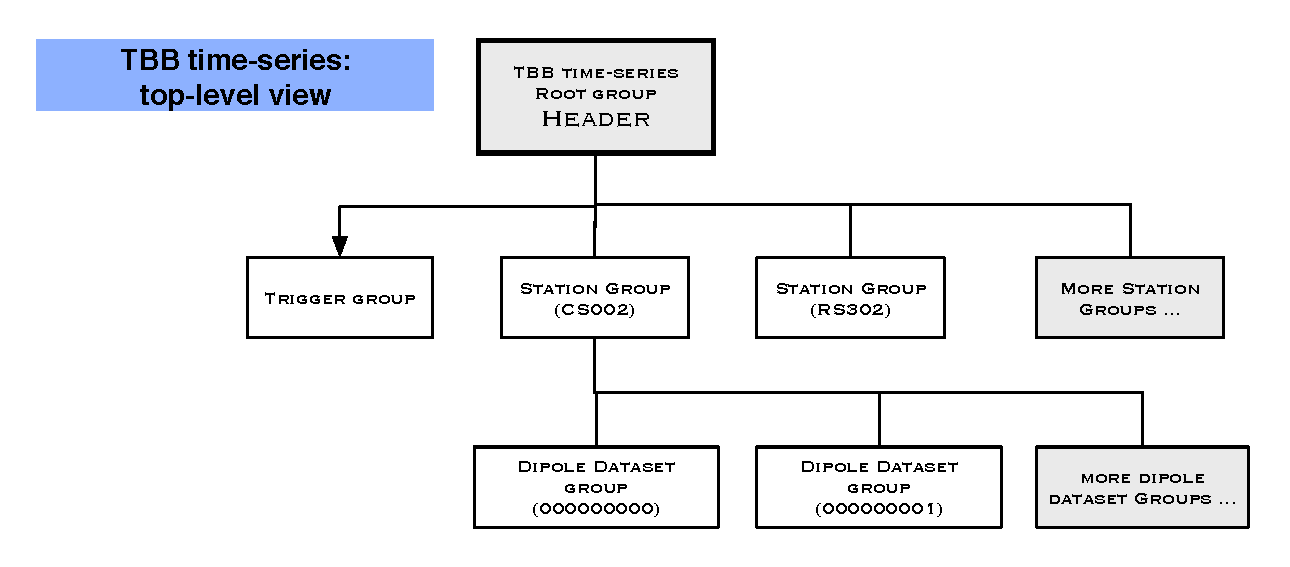
\includegraphics[width=\textwidth]{figures/TBB_highlevel_new.eps}
  \caption[Hierarchical structure of a TBB times-series dataset.]{
    Hierarchical structure of a TBB times-series dataset; the
    internal organization of the data follows the hierarchical
    organization of the LOFAR system.}
  \label{fig:TBB_highlevel}
\end{figure}

{\small
\begin{verbatim}
/                                          ...  Root Group
|-- TRIGGER                                ...  Group
|-- STATION_{AAKKK}                        ...  Group
|   |-- FIELD_XBA                          ...  Group (LBA or HBA)
|   |   |-- DIPOLE_{NNNMMMLLL}                 ...  Dataset     [1D, short] (Raw Voltage Mode)
\end{verbatim}
}

This structure can be represented through HDF5 as a \textsc{posix}-style hierarchy:

Raw Voltage Mode:
\begin{verbatim}
/
/TRIGGER
/STATION_CS002
/STATION_CS002/FIELD_LBA/DIPOLE_000000000
/STATION_CS002/FIELD_LBA/DIPOLE_000000001
/STATION_CS002/FIELD_LBA/DIPOLE_000...
/STATION_CS002/FIELD_HBA/DIPOLE_000000000
/STATION_CS002/FIELD_HBA/DIPOLE_000000001
/STATION_CS002/FIELD_HBA/DIPOLE_000...
/STATION_RS302
/STATION_RS302/FIELD_LBA/DIPOLE_001000000
/STATION_RS302/FIELD_LBA/DIPOLE_...
/STATION_RS302/FIELD_HBA/DIPOLE_001000000
/STATION_RS302/FIELD_HBA/DIPOLE_001...
...
\end{verbatim}


%%______________________________________________________________________________
%%                                                   Detailed Data Specification

\clearpage

\section{Detailed Data Specification}
\label{sec:detailed structure}

\input metadata_intro

\subsection{The Root Group}
\label{sec:root group}

The LOFAR file hierarchy begins with the top level \verb|`Root Group'|.  This is
the file entry point for the data, and the file node by which navigation of
the data is provided. The \texttt{Root Group} will comprise a set of attributes
that describe the underlying file structure, observational metadata, the LOFAR
TBB data, as well as providing hooks to all groups attached to the \texttt{Root
  Group}.

This section will specify two sets of attributes that will appear in
the \texttt{Root Group}: a set of \cla\ (CLA) that will be common to
all LOFAR science data products, and a set of attributes that are
specific to LOFAR TBB Time-series data.  Though these attributes will
all appear together in the \texttt{Root} attribute set, they are
separated in this document in order to demarcate those general LOFAR
attributes that are applicable across all data, and those attributes
that are TBB-specific.\\
In other words,

\begin{verse}
\verb|Root Attributes = Common LOFAR Attributes (CLA) + Supplemental TBB Root Attributes.|
\end{verse}

The \cla\ are the first attributes of any LOFAR file root group.

\subsubsection{\cla}
\label{sec:common lofar attributes}

This section will specify a set of attributes that will be common to
LOFAR science data products.  These ``common LOFAR metadata'' will
appear as attributes at the root level of all LOFAR data files.
\textit{All} LOFAR data products, including TBB Time-series
\textit{inter alia,} will share a common set of metadata root-level
attributes.  These common LOFAR metadata are to be the first set of
attributes of any LOFAR file root group.

Table~\ref{tab:lofar common metadata} lists the {\cla} (CLA) which can
be found in LOFAR observation mode data types: Beam-Formed, Transient
Buffer Board (TBB) dumps, Time-series, and Sky Images within the
files' root header. These Attributes are required to be in the Root
Group; if a value is not available for an Attribute, a \verb|`NULL'|
maybe used in its place.

\begin{table}[tbp]
  \centering
  \begin{tabular}{|lrp{6cm}|}
    \hline
    \textsc{General LOFAR Group} & \textsc{Value} & \textsc{Description} \\
    \hline
    Root          & \verb|`Root'|    & Top-level LOFAR group type.\\
    \hline
    \hline
    \textsc{TBB Specific Groups} & \textsc{Value} & \textsc{Description} \\
    \hline
    
    Trigger group & \verb|`TriggerGroup'| &  Trigger data group. \\
    Station group & \verb|`StationGroup'| & Station data group. \\
    Field group & \verb|`FieldGroup'|  & Antenna Field data group. \\
    Dipole dataset & \verb|`DipoleDataset'| & Individual Dipole Dataset (Raw Voltage Mode). \\
    Calibration table & \verb|`CalibrationTable'| & Table (station) calibration data. \\
    % Source group & \verb|`Source'| & This is a Source List group. \\
    % Processing History group &\verb|`ProcessHist'| & This is a Processing History group. \\
    % \textbf{Coordinates Group} & \verb|`Coordinates'| & This is a Coordinates group. \\
    % \hline
    % \textsc{Coordinates Group Subgroups} & \textsc{Value} & \textsc{Description} \\
    % \hline
    % Time coord group		&\verb|`TimeCoord'|		& Describes a time axis. \\
    % Direction coord group	&\verb|`DirectionCoord'|	& Describes a direction group. \\
    % Spectral coord group	&\verb|`SpectralCoord'|		& Describes a frequency group. \\
    \hline
  \end{tabular}
  \caption{LOFAR TBB Time-series Group Types.}
  \label{tab:group types}
\end{table}

\input lofar_common_metadata


\subsubsection{Additional TBB Time-series Root Attributes}
\label{sec:additional root group attributes}

As explained at the beginning of Sec.~\ref{sec:root group} above, the
root group of a \textbf{TBB Time-series data file} will contain a set
of attributes, which can be broken down into two subsets: 1) a set of
\cla\ (CLA) that will be common to all LOFAR science data products,
and 2) a set of attributes that are specific to LOFAR Time-series data
(see Table~\ref{tab:hdf5 root group}). With the {\cla} already listed
in section~\ref{sec:common lofar attributes} above, this section will
focus on the second subset of root group attributes, as they are
specific to a \textbf{TBB Times-series data file}.

\begin{table}[htbp]
  \centering
  \begin{tabular}{|llp{9cm}|}
    \hline
    \textsc{Field/Keyword} & \textsc{Type} & \textsc{Description} \\
    \hline
    \hline
    \verb|OPERATING_MODE| & \verb|string| & Can either be ``transient'' or
    ``spectral'', The latter is not supported in DAL / TBB Writer v2.5(.0) \\
    \verb|NOF_STATIONS| & \verb|unsigned| &  The number of station groups
    available in the file.\\
    \verb|STATION_{AAKKK}| & Group & Station group collecting the data
    from an individual LOFAR station; the station name consists of 2
    characters (upper case) and three digits.\\
    \verb|TRIGGER| & Group & Group collecting the
    parameters associated with the trigger and the output
    parameters generated by it. \\
    \hline
  \end{tabular}
  \caption{Additional attributes and objects attached to the root
    group of a TBB time-series data file.}
  \label{tab:hdf5 root group}
\end{table}

\begin{comment}
OPERATING\_MODE seems to not be really well defined.
"transient" = raw voltage mode? 
"spectral" = subband mode? Both are transient modes. Renaming things might break existing readers.
\end{comment}

\clearpage

%%_______________________________________________________________________________
%%                                                    Station Group 

\subsection{The Station Group}
\label{sec:station group}

Given the different modes for cosmic ray observation, a single LOFAR
station is the natural choice for a first grouping of time-series
data from the individual dipoles; for that matter we consider the
\textbf{station group} (Table~\ref{tab:station group}) as a basic module within
the data structure.\footnote{Though from initial perception the described
structure can be perceived as a table, the HDF5 internal data model is that
of a group; in order to stick as closely as possible to the libraries naming
conventions, we therefore use the name \textsl{group} instead of \textsl{table}.}
Creating a snapshot of multiple stations, or even the full LOFAR array, thus will
result in a set of station groups -- which in turn might be collected into
another superstructure.

\begin{table}[htbp]
  \centering
  \begin{tabular}{|llllp{4.5cm}|}
    \hline
    \textsc{Field/Keyword} & \textsc{H5Type} & \textsc{Type} & \textsc{Software} & \textsc{Description} \\
                           &                 &               & \textsc{Version}  &                      \\
    \hline
    \hline
    \small {\texttt{GROUPTYPE}} & Attr & \verb|string| & DAL v2.0 & LOFAR group type, \texttt{StationGroup}. \\
    \small {\texttt{STATION\_NAME}} & Attr & \verb|string| & DAL v2.0 & The name of the station, consisting of two characters (upper case) and three digits, e.g. \texttt{CS001} or \texttt{RS201}. \\
    \small {\texttt{FIELD\_XBAX}} & Group & --- & DAL v4.0 & Container group for dipole datasets per antenna field; The name is either \texttt{FIELD\_LBA} for the low band antennas or \texttt{FIELD\_\HBA}, \texttt{FIELD\_\HBA0}, or \texttt{FIELD\_\HBA1} for the high band antennas. \\
    \hline
  \end{tabular}
  \caption[Fields in the station data group (\texttt{StationGroup}).]{
    Fields in the station data group (\texttt{StationGroup}). The
    main purpose of this group of to serve as a common container for the separate
    sub-tables, which take up data from the TBB. Shapes of vector and matrices are given in
    \texttt{[ ]}-brackets in the description. See text for detailed explanation
    on the individual fields in the table.}
    
  \label{tab:station group}
\end{table}


\subsection{The Field Group}
\label{sec:field group}

With LOFAR 2.0, both the LBA and HBA antenna fields can be active at the same time and with different settings. Therefore we divide the \texttt{StationGroup} into \texttt{FieldGroup} first and move field specific keywords here compared to the LOFAR1 TBB Time-Series Data format. Before, most of these keywords could be found in the \texttt{StationGroup}.

\begin{table}[htbp]
  \centering
  \begin{tabular}{|llllp{4.5cm}|}
    \hline
    \textsc{Field/Keyword} & \textsc{H5Type} & \textsc{Type} & \textsc{Software} & \textsc{Description} \\
                           &                 &               & \textsc{Version}  &                      \\
    \hline
    \hline
    \small {\texttt{GROUPTYPE}} & Attr & \verb|string| & DAL v4.0 & LOFAR group type, \texttt{StationGroup}. \\
    \small {\texttt{STATION\_POSITION}} & Attr & \verb|array<double,1>| & DAL v4.0 & [3] Numerical value of the station position coordinates of this antenna field. \\
    \small {\texttt{STATION\_POSITION\_UNIT}}  & Attr & \verb|string| & DAL v4.0 & Physical units associated with the numerical values for the station position. \\
    \small {\texttt{STATION\_POSITION\_FRAME}} & Attr & \verb|string| & DAL v4.0 & Identifier for the reference frame within which the station position is provided. \\
    \small {\texttt{BEAM\_DIRECTION}} & Attr & \verb|array<double,1>| & DAL v4.0 & [2] Numercial value of the station-beam direction for this antenna field. \\
    \small {\texttt{BEAM\_DIRECTION\_UNIT}}  & Attr & \verb|string| & DAL v4.0 & Physical units associated with the numerical value of the station-beam direction. Mandatory for \verb|HBA| station data.\\
    \small {\texttt{BEAM\_DIRECTION\_FRAME}} & Attr & \verb|string| & DAL v4.0 & Identifier for the reference frame within which the station-beam direction is provided. Mandatory for \verb|HBA| station data.\\
    \small {\texttt{CLOCK\_OFFSET}} & Attr & \verb|double| & DAL v4.0 & (Relative) Station clock offset. \\
    \small {\texttt{CLOCK\_OFFSET\_UNIT}} & Attr & \verb|string| & DAL v4.0 & Physical unit for the station clock offset. \\
    % \small \textit{\texttt{TRIGGER\_OFFSET}} & Attr & \verb|double| & DAL v2.0 & Trigger time -- in seconds -- relative to the reference time. \\
    \small {\texttt{NOF\_DIPOLES}} & Attr & \verb|unsigned int| & DAL v4.0 & The number of dipoles, for which data are embedded within this group. \\
    \hline
    \small \textit{\texttt{STATION\_CALIBRATION}} & Group & --- & DAL v4.0 & Calibration information as delivered through the online (station) calibration. \\
    \small {\texttt{DIPOLE\_\{NNNMMMLLL\}\}}} & Dataset & \verb|array<short,1>| & DAL v4.0 & Dataset containing the actual raw samples read out from the transient buffer; the name of the dataset is constructed from the \small \textit{\texttt{STATION\_ID}} (NNN), \verb|RSP_ID| (MMM) and \verb|RCU_ID| (LLL) \\
  \end{tabular}
  \caption[Fields in the field data group (\texttt{FieldGroup}).]{
    Fields in the field data group (\texttt{FieldGroup}). The
    main purpose of this group of to serve as a common container for the separate
    sub-tables, which take up data from the TBB. Shapes of vector and matrices are given in
    \texttt{[ ]}-brackets in the description. See text for detailed explanation
    on the individual fields in the table.}
  \label{tab:field group}
\end{table}

The following entries will be found in the station group (Table~\ref{tab:station group}, p.~\pageref{tab:station group}):
\begin{list}{\textbf{--}}{}
\item \verb|GROUPTYPE| identifies the group as a \verb|StationGroup|.
\item While an internal identifier for the station is provided
  through the station ID, for better diagnostics the actual name of
  the station will be required; therefore \verb|STATION_NAME| will
  store the actual name of the station, e.g. \texttt{CS001},
  \texttt{RS201} or \texttt{DE602}.
\item The \textbf{position of the LOFAR station} is reconstructed from the three
  attributes
  \begin{itemize} \parskip 0pt
  \item \verb|STATION_POSITION| -- numerical value of the station position
    coordinates
  \item \verb|STATION_POSITION_UNIT| -- physical units associated with the numerical
    values for the station position
  \item \verb|STATION_POSITION_FRAME| -- identifier for the reference frame within
    which the station position is provided
  \end{itemize}
\item The \textbf{direction of the Tile Beam} on top of which the observation
  potentially has been running in piggy-back mode:
  \begin{itemize} \parskip 0pt
  \item \verb|BEAM_DIRECTION| -- numerical value of the Tile Beam
    direction. This is the same as the direction of the first Sub Array Pointing and Station Beam. \footnote{Please note that as of writing in 2018, the Tile Beam, SAP0 and the Station Beam will all have the same pointing/direction, but LOFAR might become more flexible in the future with LOFAR 2}
  \item \verb|BEAM_DIRECTION_UNIT| -- physical units associated with the numerical
    value of the Tile Beam direction
  \item \verb|BEAM_DIRECTION_FRAME| -- identifier for the reference frame within
    which the Tile Beam direction is provided
  \end{itemize}
\item \verb|NOF_DIPOLES| is a counter for the number of dipoles, for which data
  are embedded within this group.
\end{list}

Even though there exist multiple LOFAR observation modes for TBBs, all
have in common a (multi-level) pulse-detection and trigger-generation algorithm;
the control parameters of the trigger algorithms as well as its output, in case
a trigger condition was derived, need to be stored.

\clearpage




\section{Data Discovery}
This section describes required/used data for discovery and related information.

\subsection{Metadata for Discovery}
The following metadata is used for discovery of data in the archive. %TODO is this not in the table?

\subsection{Data size calculation}

The general data size calculation for TBuf data is:

Number of stations x number of antennas per station x Duration (s) x (200000000) samples per second x 8 Bytes per sample

We neglect the metadata as it is small in comparison.


Use cases: The data format needs to be able to handle data volumes as different as a
CR event with 1ms worth of data from a few antennas only to a full dump of 1
second worth of data from all LOFAR antennas in a consistent and efficient way.

\begin{description}
\item[UHEP-mode:]\ \\[2mm]
  \sumline{Time series data from the formed beam\\
    $ \hbox{2 pol} \times
    2^{27} \hbox{ samples} \times
    8 \hbox{ Bytes/sample}$:}{\\2.0\,GB/event}
  \sumline{Raw time series data from individual dipoles\\
    $  77 \hbox{ stations} \times
    48 \hbox{ antennae} \times
    2 \hbox{ pol} \times
    2^{17} \hbox{ samples} \times
    2 \hbox{ Bytes/sample}$:}{\\\underline{1.8\,GB/event}}
  \sumline{Total:}{3.8\,GB/event}
\item[VHECR-mode:]\ \\[2mm]
  \sumline{Raw time series data from individual dipoles\\
   % $ 32 \hbox{ core stations} \times
    $48 \hbox{ antennae} \times
    2 \hbox { pol} \times
    2^{17} \hbox{ samples} \times
    2 \hbox{ Bytes/sample}$:}{\\25\,MB/event}
\item[HECR-mode:]\ \\[2mm]
  \sumline{Similar, but now only one station is involved\\
    $ 48 \hbox{ antennae} \times
    2 \hbox { pol} \times
    2^{17} \hbox{ samples} \times
    2 \hbox{ Bytes/sample}$:}{\\25\,MB/event}
\item[TS-mode:]\ \\[2mm]
  \sumline{Similar to VHECR but full raw data from TBB\\
    $ 77 \hbox{ stations} \times
    48 \hbox{ antennae} \times
    2 \hbox{ pol} \times
    2 \cdot 10^{8} \hbox{ samples} \times
    2 \hbox{ Bytes/sample}$:}{\\3.0\,TB/event}
\end{description}

The event rate is uncertain, and for VHECR is estimated at one triggered event per station
per 10 minutes. With 32 stations active this would amount to 110 GB per day of observing time.


%% ------------------------------------------------------------------- References
\section{References}

\subsection{Common LOFAR2 attributes}

\subsection{Naming conventions}

\bibliographystyle{abbrv}
\bibliography{references}


%%_______________________________________________________________________________
%%                                                    Discussion & open questions

\clearpage

\appendix
\section{Appendix}

\subsection{Glossary}
\label{sec:glossary}
\addcontentsline{toc}{section}{\glossaryname}

\input lofar_common_glossary


\subsection{Data Types}

\subsection{Notation}

\subsection{FAQ/known issues}


\subsection{Discussion \& open questions - remove before publication}

The following table presents an overview of (some of the) known open
questions regarding the format definition:

\begin{center}
  \tablefirsthead{
    \hline
    \textsc{Item} & \textsc{Description} & \textsc{Raised by} \\
    \hline
  }
  \tablehead{
   \multicolumn{3}{r}{\small\textsl{continued from previous page}} \\
    \hline
    \textsc{Item} & \textsc{Description} & \textsc{Raised by} \\
    \hline
  }
  \tabletail{
    \hline
    \multicolumn{3}{r}{\small\textsl{continued on next page}} \\
 }
  \tablelasttail{\hline}
  \begin{supertabular}{lp{12.8cm}l}
    01 & Are there modes forseen in which the total LOFAR array is being split up
    into sub-arrays operating in different modes? In such a case the
    \textsl{range of application} of some of the metadata
    keywords would change; in order not to shift keywords within the data structure
    we therefore will end up with redundant information, depending of the specific
    observation mode. The latter though will not pose a major problem, since this
    redundance will show up in non-datasize critical keywords, such e.g.
    \verb|OBSERVATION_MODE| or \verb|NYQUIST_ZONE|. & L.\ Baehren \\
    02 & How to handle multiple HBA tile beams per station? Perhaps via subgroups of the dipole group? & L.\ Baehren \\
    03 & Is there indeed a separate value available which describes
    the conversion from ADC counts to voltages, or is this part of the
    gain calibration? If the latter is the case, then how to get a
    voltage time-series? & L.\ Baehren \\
    04 & Currently the trigger meta-data has no defined format. In the
    future, there will be a specific format for each trigger mode,
    i.e.\ an `UHEP' group etc. In the meantime, the current format is
    to be used as a long character string that can be used flexibly. & C. James \\
    05 & With LOFAR 2.0 the data is now divided into \texttt{StationGroup} with \texttt{FieldGroup} subgroups. The alternative would be to include the Field in the \texttt{StationGroup} name and add a keyword for the antenna field. This is more consistent with the LOFAR 1 dataformat. Would that be better? & S. ter Veen \\
    06 & Should PROJECT\_PI, CO\_I, CONTACT name be removed because of GDPR? & S. ter Veen \\
    07 & Is \texttt{SYSTEM\_VERSION} enough distinction between LOFAR1 and LOFAR2? Should there be a different keyword or file extension (tbuf) & S. ter Veen \\
 \end{supertabular}
\end{center}

\subsection{Future enhancements}

Though the file format definition is not intended to undergo
considerable changes once gaining release status, there will be future
enhancements to reflect new insights and address noted short-comings.

\begin{enumerate}
\item Some additional metadata are required when the observation is
  done using the HBA [input thanks to Maaijke Mevius]:
  \begin{enumerate}
  \item At station level the 4x4 numbers which give the relative
    position of the dipoles in a tile, given in HBADeltas.conf. We do
    not really need those for analysis, but if you want to simulate
    the data (or do some sort of selfcal) it might be good to have
    them. \\
    Since these numbers are the same for all tiles within a station, I
    think they can be stored in the station metadata.
  \item The pointing of the tile beam (2 angles) should be added. I
    believe it is possible to have different tiles pointing in
    different directions, thus it should be stored per antenna.
  \item By `tiles', do we mean literal tiles, or tiles/dipoles? [CWJ]
  \end{enumerate}
\end{enumerate}

%%_______________________________________________________________________________
%%                                                                     Appendices

\clearpage

\section{Document history}
\addcontentsline{toc}{section}{Change record}


\subsection{Version 1.x}

\subsubsection*{Notes for Version 1.0 $\rightarrow$ Version 1.1}

\begin{enumerate}
\item \textit{Reorganisation of the placement of attributes describing
    basic properties of the observation from which the dataset has
    originated.} \\
  Some part of the information which originally was supposed to be stored within
  the Station groups should be shifted upwards to the root group of the file.
  \begin{itemize}
  \item[\underline{old}:]
    {\small
\begin{verbatim}
/
|-- STATION_001                         ... Group
|   |-- TELESCOPE                       ... Attribute       ... string
|   |-- OBSERVER                        ... Attribute       ... string
|   |-- PROJECT                         ... Attribute       ... string
|   |-- OBSERVATION_ID                  ... Attribute       ... string
|   |-- OBSERVATION_MODE                ... Attribute       ... string
|   `
|-- STATION_002                         ... Group
|   |-- TELESCOPE                       ... Attribute       ... string
|   |-- OBSERVER                        ... Attribute       ... string
|   |-- PROJECT                         ... Attribute       ... string
|   |-- OBSERVATION_ID                  ... Attribute       ... string
|   |-- OBSERVATION_MODE                ... Attribute       ... string
|   `
\end{verbatim}}
  \item[\underline{new}:]
    {\small
\begin{verbatim}
/
|-- TELESCOPE                           ... Attribute       ... string
|-- OBSERVER                            ... Attribute       ... string
|-- PROJECT                             ... Attribute       ... string
|-- OBSERVATION_ID                      ... Attribute       ... string
|-- OBSERVATION_MODE                    ... Attribute       ... string
|-- STATION_001                         ... Group
|   |
|   `
|-- STATION_002                         ... Group
|   |
|   `
\end{verbatim}}
  \end{itemize}
\item \textit{Proper handling of coordinates} \\
    The motivation for this changes are in the fact, that for proper
    representation of a direction or position information more but just the
    numerical value is required -- thus the additional information should be
    stored within the file as well, as compared to simply assuming the stored
    data adhere to a certain convention (which on the other hand they still
    should).
  \begin{itemize}
  \item[\underline{old}:]
    {\small
\begin{verbatim}
/
|-- STATION_001                         ... Group
|   |-- BEAM_DIRECTION                  ... Attribute       ... array<double,1>
|   |-- 001000000                       ... Dataset
|   |   |-- ANTENNA_POSITION            ... Attribute       ... array<double,1>
|   |   |-- ANTENNA_ORIENTATION         ... Attribute       ... array<double,1>
|   |   |-- SAMPLE_FREQUENCY            ... Attribute       ... double
|
\end{verbatim}}
  \item[\underline{new}:]
    {\small
\begin{verbatim}
/
|-- STATION_001                         ... Group
|   |-- STATION_POSITION_VALUE          ... Attribute       ... array<double,1>
|   |-- STATION_POSITION_UNIT           ... Attribute       ... string
|   |-- STATION_POSITION_FRAME          ... Attribute       ... string
|   |-- BEAM_DIRECTION_VALUE            ... Attribute       ... array<double,1>
|   |-- BEAM_DIRECTION_UNIT             ... Attribute       ... string
|   |-- BEAM_DIRECTION_FRAME            ... Attribute       ... string
|   |-- 001000000                       ... Dataset
|   |   |-- ANTENNA_POSITION_VALUE      ... Attribute       ... array<double,1>
|   |   |-- ANTENNA_POSITION_UNIT       ... Attribute       ... string
|   |   |-- ANTENNA_POSITION_FRAME      ... Attribute       ... string
|   |   |-- ANTENNA_ORIENTATION_VALUE   ... Attribute       ... array<double,1>
|   |   |-- ANTENNA_ORIENTATION_UNIT    ... Attribute       ... string
|   |   |-- ANTENNA_ORIENTATION_FRAME   ... Attribute       ... string
|   |   |-- SAMPLE_FREQUENCY_VALUE      ... Attribute       ... double
|   |   |-- SAMPLE_FREQUENCY_UNIT       ... Attribute       ... string
|
\end{verbatim}}
  \end{itemize}
\item \textit{Sensible (default) values} \\
  One of the -- at least temporary -- problems is, that some of the values to be
  stored within the HDF5 file are not available (yet) at the time of creating the
  file on disk. Therefore at least sensible default values/settings should be used
  to enable correct interpretation of the dataset; e.g. position information at a
  later point will be retrieved from the central parameter database, but until then
  the attributes should be filled already with placeholder values which agree with
  the conventions of the Measures framework. If a value in fact is undefined, it
  should be clearly marked as such by using \verb|UNDEFINED| (in case of a string
  valued attribute).
  {\small
\begin{verbatim}
/
|-- STATION_001
|   |-- STATION_POSITION_VALUE         ... array<double,1>    ...  {x,y,z}
|   |-- STATION_POSITION_UNIT          ... string             ...  "m"
|   |-- STATION_POSITION_FRAME         ... string             ...  "ITRF"
|   |-- BEAM_DIRECTION_VALUE           ... array<double,1>    ...  {0,90}
|   |-- BEAM_DIRECTION_UNIT            ... string             ...  "deg"
|   |-- BEAM_DIRECTION_STRING          ... string             ...  "UNDEFINED"
|   |-- 001000000
|   |   |-- ANTENNA_POSITION_VALUE     ... array<double,1>    ...  {x,y,z}
|   |   |-- ANTENNA_POSITION_UNIT      ... string             ...  "m"
|   |   |-- ANTENNA_POSITION_FRAME     ... string             ...  "ITRF"
|   |   |-- ANTENNA_ORIENTATION_VALUE  ... array<double,1>    ...  {x,y,z}
|   |   |-- ANTENNA_ORIENTATION_UNIT   ... string             ...  "m"
|   |   |-- ANTENNA_ORIENTATION_FRAME  ... string             ...  "ITRF"
|   |   |-- FEED                       ... string             ...  "UNDEFINED"
|   |   |-- NYQUIST_ZONE               ... uint               ...  1
|   |   |-- SAMPLE_FREQUENCY_UNIT      ... string             ...  "Hz"
|
\end{verbatim}}
\end{enumerate}




\subsubsection*{Version 4.0 $\rightarrow$ Version 4.x}

\begin{center}
  %% Table head
  \tablefirsthead{
    \hline
    \textsc{Version} & \textsc{Date} & \textsc{Sections} & \textsc{Description of changes} \\
    \hline
  }
  \tablehead{
    \multicolumn{4}{r}{\small\textsl{continued from previous page}} \\
    \hline
    \textsc{Version} & \textsc{Date} & \textsc{Sections} & \textsc{Description of changes} \\
    \hline
  }
  %% Table tail
  \tabletail{
    \hline
    \multicolumn{4}{r}{\small\textsl{continued on next page}} \\
  }
  \tablelasttail{\hline}
  %% Table contents
  \begin{supertabular}{lllp{9.5cm}}
    4.00.00 & 2025-06-13 & all   & Changes for LOFAR2.0. Removed Subband Groups. Introduced \texttt{FieldGroup}. Added keyword \texttt{TILE\_DIPOLES\_ENABLED}. Moved \texttt{DIPOLE\_CALIBRATION} values to a separate group where calibration table can be stored. \\
    4.01.00 & 2018-10-24 & all   & Cleanup of the document. \\
 \end{supertabular}
\end{center}


\subsection{Metadata}
\label{sec:metadata}

Metadata is the auxiliary data stored along with the time series data need to
provide all the necessary information for automated processing of the data.
This data can either be stored directly in the data set or it can be stored
in an external database. In the latter case the data set must contain a
pointer to the correct entry in that database (e.g. the antenna-id is needed
to get the antenna position).

\begin{itemize} \parskip 0pt
\item DAQ mode, including Samplerate, Filters, etc.
\item Timing information:
  \begin{itemize}
  \item Trigger time relative to recorded data segement
  \item Timing of the data streams relative to the trigger
  \item Timing of the data streams relative to each other with sub-sample
    accuracy; This can be implicit, e.g. all data streams of a station start
    at the same time. Fields that can be in stored in an external database.
  \end{itemize}
\item List of RFI sources identified by the station calibration, including
  \textbf{direction}, \textbf{center frequency} and \textbf{peak strength}.
  \begin{list}{$\rightarrow$}{}
  \item What does this actually mean: the properties of the single channel
    containing the highest signal level or the parameters obtained from fitting
    e.g. a Gaussian to a segment of the spectrum?
  \end{list}
\item Dispersion measure of the ionosphere (at this point in time and space)
\item Health information about the antennas
\end{itemize}

\subsubsection{System monitoring and system health.}

Information on the status of the various (hardware) components at a LOFAR station
will be stored inside the PVSS database; a description of the datapoint-types and
datapoints can be found in the \verb|MAC/Deployment/data/PVSS| branch of the
LOFAR code repository (see Table~\ref{tab:PVSS} for an excerpt).

\begin{table}[htb]
  \centering
  \begin{tabular}{|lll|}
    \hline
    \textsc{Database entry} & \textsc{Field} & \textsc{Format} \\
    \hline
    \hline
    CalCtlr & connected    & unsigned int \\
            & obsname      & string \\
            & antennaArray & string \\
            & filter       & string \\
            & nyquistzone  & int \\
            & rcus         & string \\
    \hline
    ObservationControl & claimPeriod & int \\
    & preparePeriod   & int \\
    & startTime       & string \\
    & stopTime        & string \\
    & subbandList     & string \\
    & beamletList     & string \\
    & bandFilter      & string \\
    & nyquistzone     & int \\
    & antenneArray    & string \\
    & receiverList    & string \\
    & sampleClock     & int \\
    & measurementSet  & string \\
    & stationList     & string \\
    & inputNodeList   & string \\
    & BGLNodeList     & string \\
    & storageNodeList & string \\
    \hline
  \end{tabular}
  \caption[Excerpt from the list of entries into the PVSS database.]{
    Excerpt from the list of entries into the PVSS database. The
    definitions of the datapointtypes and datapoints can be found in the
    \texttt{MAC/Development/data/PVSS} branch of the LOFAR code repository.}
  \label{tab:PVSS}
\end{table}

In order to later store certain system health information along with the other
data, parameters need to be subscribed to at the definition of the observation.

\subsection{Visualization}

Past experience with the software for the LOPES experiment has shown, that is
is crucial to provide the user with a variety of way to graphically inspect
the data. This not only includes visualization of the time-series/FFT/etc.
data themselves, but also displaying the various data with the wider context
of the experimental setup (e.g. geographical distribution of the antennas
w.r.t. to the particle detector setup)

\begin{itemize}
\item Display of the standard data products (also see documentation of the
  \lopestools\ \verb|DataReader|): ADC, Voltage, FFT, Calibrated FFT,
  RFI-filtered FFT, Cross-Corr. Spectra, Visibilities
\item Display of the (intermediate) data products generated from the input
  data, e.g. dynamic spectra, multi-dimensional skymaps
\item Flags and weights associated with the data, e.g. filter curves, antenna
  gain curves, etc.
\item Station layout, i.e. positions of the (selected/excluded) antennas
\item antenna power level distribution over the area of the station/array
  (this is very similar to the type of event display as known from particle
  physics experiments)
\item mapping of the (local) RFI via an (Azimuth,Frequency) plot centered on
  the position of a certain station
\item geographical locations of identified RFI sources; such a plot should
  also indicate the  frequency band of the RFI (via label or bar etc.)
\item geographical distribution/location of antennas which generated a trigger
  signal, failed, etc.
  \begin{itemize}
  \item[$\rightarrow$] VR setting, combining geographical information (e.g.
    map of the Netherlands) with the location of localized CR-/TS-events
  \item[$\Rightarrow$] in a cave-like setup we actually can perform a
  fly-through, which would be ideal for outreach purposes!
  \end{itemize}
\item cummulative geographical distribution of detected CR events
\item total power per LOFAR station (geographically distributed)
\item overlay of CR data with information from other sensors (e.g. weather
  radar images, temperatures, etc.)
\end{itemize}
A number of the before-mentioned displayes should be interactive, in the sense
that the user should be able to perform data selection from the graphical
display (e.g. by drawing a circle around the core of the CR air shower,
thereby selecting the antennas included in the data analysis step).





\end{document}
